\chapter{Practical application of DFT}
\label{sec:Practical DFT}

In this section we will present the practical application and implementation of density functional theory in the study of materials science.

\section{The Exchange-Correlation functional}
\textbf{\cite{xc_bandgap} is a good reference for the results regarding the band gap of different solids for a number of functionals}

From the former section, we know that the only peace of information we require to perform DFT plane-wave calculations are that of the exchange-correlation energy $E_{\text{xc}}[n]$. Only for a homogeneous electron gas (HEG) is the exact exchange-correlation energy known. The HEG is of limited use in practical application considering that the variation in the electronic concentration is responsible for a wide range of properties. However, the local density approximation (LDA) have found large sucsess from building on the HEG. In the LDA, $E_{\text{xc}}[n]$ is  approximated by an electron in an homogeneous electron gas of density $n(\boldsymbol{r})$ .  

\begin{equation}
    E_{\text{xc}}^{\text{LDA}}[n(\boldsymbol{r})] = \int n(\boldsymbol{r})\epsilon_{\text{xc}}[n(\boldsymbol{r})]d\boldsymbol{r}.
\end{equation}

The success of this approach is most dominant in systems with slowly varying charge density, ie bulk materials. A notable downside of LDA is the degree of self-interaction, by only including the local environment, which lead to artificial contributions to the electron density. A significant upside of this method is the low computational cost. \textbf{More on LDA?}

A natural succession to the local density approximation is the family of generalized gradient approximation (GGA).  

\begin{equation}
  E_{\text{xc}}^{\text{GGA}}[n(\boldsymbol{r})] = \int f(n(\boldsymbol{r}), \nabla n(\boldsymbol{r}))d\boldsymbol{r}.
\end{equation}

GGA improves on LDA by additonly considering the gradient of the electron concentration. There currently exists many approaches for how to construct the function $f$ to include the gradient, the two most common are Perdew-Wang 91 (PW91) \cite{pw91} and Perdew-Burke-Ernzerhof (PBE) \cite{pbe}. 

Further, we can extended this idea to include the laplacian $\nabla^2$ of the density. This range of methods is called meta-GGA, popular implementations include \textit{Modified Becke and Johnson} (MBJ) \cite{mbj} and \textit{Strongly Constrained Appropriately Normed} (SCAN) \cite{scan}. \textbf{Write a brief discussion of these, see for example \cite{scan2}}.

Very precise calculations can be obtained from combining LDA/GGA with the exact Hartree-Fock exchange energy. This method was proposed by Becke as hybrid functionals, since the functional is a hybrid between the two. \textbf{Insert eq for hybrid functionals?} This method is superior in describing localized states, but comes at a significant larger computational cost. In order to reduce this cost, Heyd al et. split the Hartree-Fock exchange into short-range and long-range parts, in which calculations can adapt exact Hartree-Fock exchange for short-range (SL) and non-exact for long-range (LR). By introducing the parameter $\omega$ to adjust the order parameter of the method, we can express this method, called HSE (Heyd-Scuseria-Ernzerhof) \cite{hse06} as
\begin{equation}
    E_{xc}^{HSE} = \alpha E_{x}^{HF,SR}(\omega) + (1-\alpha)E_{x}^{PBE, SR}(\omega) + E_x^{PBE,LR}(\omega) + E_{c}^{PBE}
\end{equation}
\textbf{Explain what the different notations mean}
\textbf{Write more/better on hybrid functionals and HSE06, see references \cite{hf_bandgap}, \cite{hf_comparision}. \cite{hse} and write a summary of the different approximations}

Over the last 50 years, over 500 different approximations have come to fruition, but mainly PBE GGA, and HSE06 have found wide-spread application and usage \cite{xc_bandgap}.

\section{Fundamental aspects of practical DFT calculations}
\textbf{Needs work, see mainly DFT book ch 3}
With the exchange-correlation functionals presented above, we now have everything in order to perform DFT calculations. To begin solving eq .., we need the single-electron wave-function, for a free electron this is a plane wave $\psi_k = Ae^{i\boldsymbol{k}\boldsymbol{r}}$. In a solid however, there exist a nonzero periodic potential $V(\boldsymbol{r}) = V(\boldsymbol{r} + \boldsymbol{R})$, the solution to the Shr\"{o}dinger equation is given by Bloch's theorem wich states that the solution takes the form
\begin{equation}
\psi_{\boldsymbol{k}}(\boldsymbol{r}) = u_{\boldsymbol{k}}(\boldsymbol{r})e^{i\boldsymbol{k}\boldsymbol{r}},    
\end{equation}
where $u_{\boldsymbol{k}}(\boldsymbol{r})$ is a bloch wave with the periodicity of the supercell, and $\boldsymbol{k}$ is the wavevector. Similar to eq(above), k-space, or reciprocal space is useful to solve the numerous mathematical problems posed by DFT. For instance a great deal of DFT calculations revolve around solving the integral 
\begin{equation}
    g = \frac{V_{\text{cell}}}{(2\pi)^3} \int_{\text{BZ}} g(\boldsymbol{k})d\boldsymbol{k},
\end{equation}
with BZ denoting that the integral be evaluated for all $\boldsymbol{k}$ in the Brillouin zone. This integral can be approximated by evaluating the integral at a set of discrete points and summing over the points with appropriatly assigined weigts. A larger set of points leads to more exact approximations. This method is called Legendre quadrature. The method for selceting these points in reciprocal space was devolped by Monkhorst and Pack in 1976, and simply put requieres a amount of kpoints in each direction in reciprocal space, in the form $N x N x N$. Recalling that reciprocal space is inverse to regular space, supercells with equal and large dimensions converge at smaller values of N, and inversly for cells of small dimsion. In supercells with different length axis, such as hexagonal cells, we use the notation $N x N x M$, where $M$ relate to the distincntly different axis. The amount of kpoints required can be fruther reduced by utulizing the symmetry of the cell, in which we can exactly approximate the entire BZ by extending a lesser zone through symmertry. This reduced zone is appropriartly named the irreducible Brillouin zone (IBZ). 

Metals in particular requiere a large set of kpoints to acchive accurate results. This is becouse we encounter discontinuies functions in the Brillouin zone around the fermi sufrace where the states discontinusly change from occupied to non-occupied. To reduce the cost of this operatin, there are two primary methods, tetrhaedon and smearing. The idea behind the tetrahedon method is to use the discrete set of k-points to fill the reciprocal space with tethraeda and interpolate the function within each tethraeda such that the function can be integrated in the entire space rather than at discrete points. The latter approach for solving discontinuos integrals is to smear out the discontinuity and thus transforming the integral to a continous one. A good analogy to this method is the fermi-dirac function, in which a small variable $\sigma$ transform a step-functino into a continious function that can be integrated by standard methods.

In addition to the number of kpoints, there is one more distinct parameter that must be specified in DFT calculations, namely the energy cutoff, or $E_{\text{cut}}$. This parameters arise from the Bloch function described previosly. In which $u_{\boldsymbol{k}}(\boldsymbol{r})$ was a bloch wave with the same periodicity as the supercell. This implies that the wave can be expanded by a set of special plane waves as
\begin{equation}
    u_{\boldsymbol{k}}(\boldsymbol{r}) = \sum_{\boldsymbol{G}} c_{\boldsymbol{G}}e^{i\boldsymbol{G}\boldsymbol{r}},
\end{equation}
where $\boldsymbol{G}$ is the reciprocal lattice vector. Combining this with eq ..(first eq for blcoh function) we get 
\begin{equation}
    \psi_{\boldsymbol{k}}(\boldsymbol{r}) = \sum_{\boldsymbol{G}} c_{\boldsymbol{k} + \boldsymbol{G}}e^{i(\boldsymbol{k} + \boldsymbol{G})\boldsymbol{r}}
\end{equation}
The consequense from this expression is that evaluating the wavefunction of an electron at a single $k$ point demand a summation over the entirity of reciprocal space. In order to reduce this computational burden, we can introduce a maximum paramater $E_{\text{cut}}$ to cap the calculations. This is possible becouse eq ..(above) is the solution of the Shr\"{o}dinger equation with kinetic energy 
\begin{equation}
    E = \frac{\hbar^2}{2m}|\boldsymbol{k} + \boldsymbol{G}|^2.
\end{equation}
Seeing as the solution with lower energies are the most interesting, we can limit the calculations of eq ..(2 above) to solutions with energy less than $E_{\text{cut}}$ given bellow
\begin{equation}
    E_{\text{cut}} = \frac{\hbar^2}{2m}G_{\text{cut}}.
\end{equation}
Thus, we can reduce the infinitly large sum above to a much more feasable calculation in 
\begin{equation}
    \psi_{\boldsymbol{k}}(\boldsymbol{r}) = \sum_{|\boldsymbol{k} + \boldsymbol{G}| < G_{\text{cut}}} c_{\boldsymbol{k} + \boldsymbol{G}}e^{i(\boldsymbol{k} + \boldsymbol{G})\boldsymbol{r}}
\end{equation}

\textbf{A summary on kpoints and ENCUT, plus a discussion on nummerical convergence and how to select kpoints and ENCUT}


A final consideration to how DFT is applied in practise is how the core electrons are handled. Tightly bound core electrons as opposed to valene electrons demand a greater number of plane-waves to converge. The most efficient method of reducing the expenses of core-electrons are so-called pseudopotentials. This method works by approximating the electron density of the core elecrons by a constant density that mimic the properties of true ion core and core electrons. This density is then remained constant for all subsequent calculations, ie only considering the valence electrons while regarding the core electrons as frozen-in. There are currently two popular types of psudopotentials used in DFT, so-called ultrasoft psudopotentials (USPPs) devoplped by Vanderbilt, and the projecter augmented-wave (PAW) method by Bloch \cite{PAW1}, \cite{PAW2}.

\section{Self-consistent field calculation}
\textbf{Needs work, see lecture notes ch 8, book ch1}
Preceding this section, we have considered the fundamental theory of DFT and it's practical ability to model various materials. In figure \ref{sfDFT} we present the self-consistent field calculation scheme for how DFT calculations are performed. The initial problem posed by dft is that all properties rely on the density, and are dependent on each other. For instance, the effective potential is dependent on the density, which again is dependent on the eigenfunctions, that rely on the effective potential again. The cleaver approach, as seen in figure \ref{sfDFT} begin with an initial guess to the density from which we can solve the Kohn-Sham equation and obtain the corresponding eigenfunctions. Following is an iterative method where we apply the recently calculated eigenfunctions to determine a new density and repeat the procedure above. This is repeated until the total energy is converged, by an own-defined criterion. Equivalently, the optimal ionic positions can be found by a similar approach. This method is based on quasi-Newton algorithms to minimize the forces between ions. 

\begin{figure}
\centering
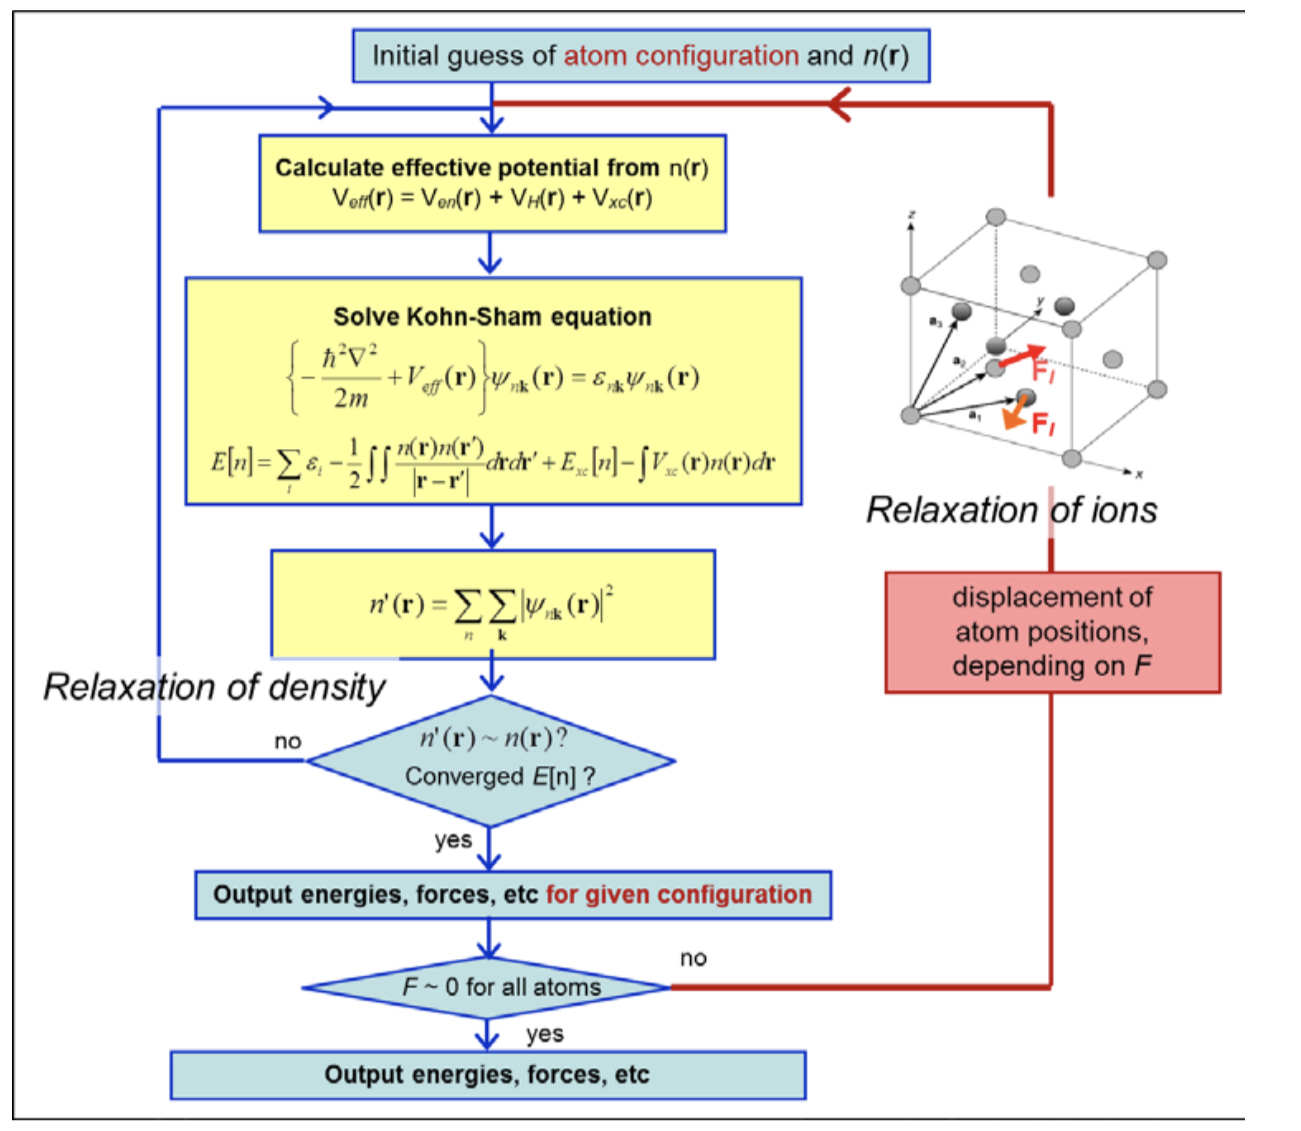
\includegraphics[scale=.3]{theory/selfConsistentDFT.jpeg}
\caption{Self consistent iteration of a DFT calculation. Figure adopted from lecture notes fys-mena4111 \textbf{cite}}
\label{sfDFT}
\end{figure}

